\documentclass[mathserif,serif]{beamer}
\usepackage{tabularx}
\setbeamertemplate{footline}[frame number]
% \useoutertheme{infolines}
\usepackage{slidesphysics}
\graphicspath{{../plot/}}

\title[]{Data/MC comparison}
\author[]
{
Samuel Lo \inst{1} \\
for SS analysis team
}
\institute[]
{
\inst{1}
The University of Hong Kong
}
\date[]{\today}

\newcommand\Wider[2][3em]{%
\makebox[\linewidth][c]{%
\begin{minipage}{\dimexpr\textwidth+#1\relax}
\raggedright
\centering#2
\end{minipage}%
}%
}

\begin{document}
\frame{\titlepage}

\begin{frame}{Introduction}
\begin{itemize}
\item Cut flow comparison
\begin{itemize}
\item The weighted number get close (within 2\%) between Daniela and me for Zmumu background. But some small difference still need to be resolved.
\url{https://docs.google.com/spreadsheets/d/12-hpz\_X154YYrYVbQPT6TL5JLWWPZa40NhN7AhhBpdc/edit\#gid=1424837111}
\end{itemize}
\item SR Optimization
\begin{itemize}
\item Comparison for with/without charge flip tagger. The Zee BG is reduced by 6 times, while the signal has small change.
\url{https://its.cern.ch/jira/browse/SUSYEWKWH-14}
\item Comparison of signal and BG in the SR of run 1
\url{https://its.cern.ch/jira/projects/SUSYEWKWH/issues/SUSYEWKWH-9?filter=allopenissues}
\end{itemize}
\end{itemize}
\end{frame}

\begin{frame}{Comparison for with/without charge flip tagger of Zee samples in CR}
CR selection
\begin{itemize}
\item same-sign two leptons
\item $|m_{ll} - 91.2| < 10$
\end{itemize}
The plot is without the mll cut. \\
The number is after the mll cut. \\
The CFT setting is used on the right plot for Zee and signal. \\
The default setting is used for VV and Vgamma for both plots. \\

\begin{columns}

\begin{column}{0.5\textwidth}
\begin{center}
\includegraphics[width=\textwidth]{mll_CR_SS_ee_Zmass_def} \\
Default: Zee: $108,072\pm1,233$
\end{center}
\end{column}

\begin{column}{0.5\textwidth}
\begin{center}
\includegraphics[width=\textwidth]{mll_CR_SS_ee_Zmass_cft} \\
CFT: Zee: $17,207\pm572$
\end{center}
\end{column}

\end{columns}

\end{frame}

\begin{frame}{Selection in run1 SR}
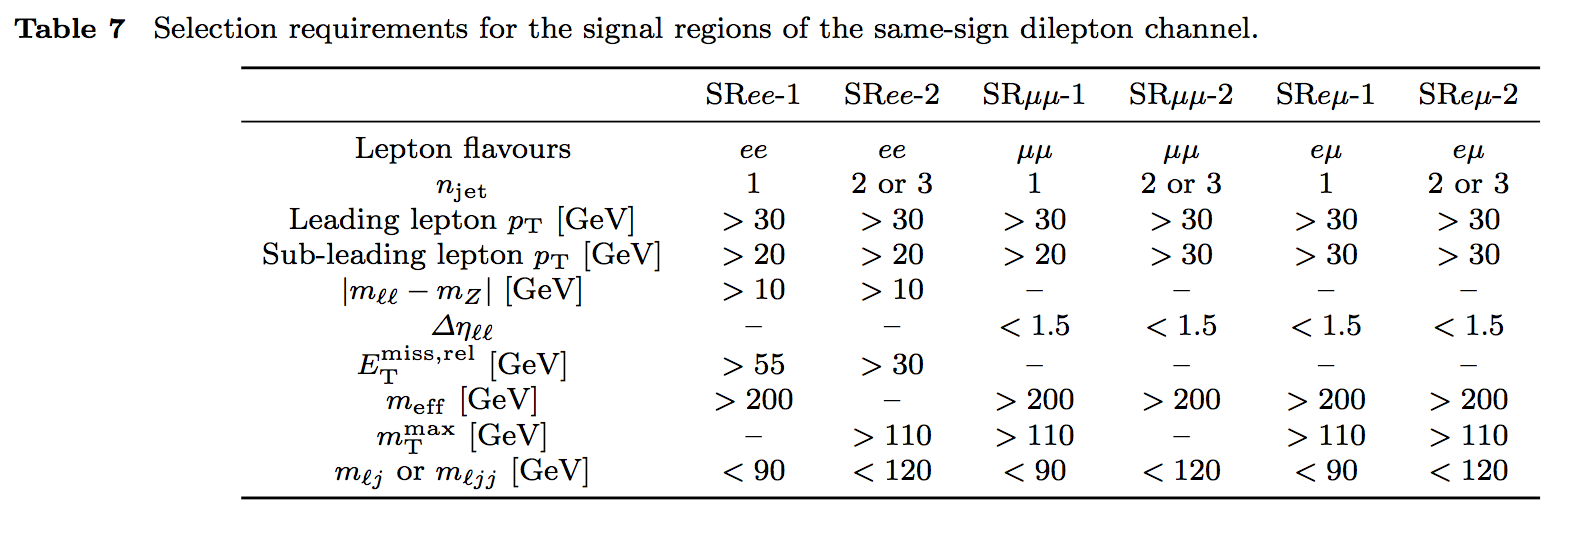
\includegraphics[width=\textwidth]{data/photo/SRcutrun1.png} \\
\url{https://arxiv.org/pdf/1501.07110.pdf}
\end{frame}

\begin{frame}{Dilepton \pt}
\begin{itemize}
\item The plot is after all run1 SR selection cut.
\item A Dilepton $\pt$ cut can be used to improve the expected significance.
\item Also checking other variables. (more plots in Backup slides)
\end{itemize}

\begin{columns}

\begin{column}{0.5\textwidth}
\begin{center}
\includegraphics[width=\textwidth]{ptll_SR_SS_ee_1} \\
SRee-1
\end{center}
\end{column}

\begin{column}{0.5\textwidth}
\begin{center}
\includegraphics[width=\textwidth]{ptll_SR_SS_mumu_1} \\
SR$\mu\mu$-1
\end{center}
\end{column}

\end{columns}

\end{frame}

\begin{frame}{Number of b-jets}
\begin{itemize}
\item Do we apply a b-jet veto?
\end{itemize}

\begin{columns}

\begin{column}{0.5\textwidth}
\begin{center}
\includegraphics[width=\textwidth]{nBJet_SR_SS_ee_1} \\
SRee-1
\end{center}
\end{column}

\begin{column}{0.5\textwidth}
\begin{center}
\includegraphics[width=\textwidth]{nBJet_SR_SS_mumu_1} \\
SR$\mu\mu$-1
\end{center}
\end{column}

\end{columns}

\end{frame}

\section{Plan}
\begin{frame}{Plan}
\begin{itemize}
\item BG composition need to be understood
\begin{itemize}
\item large contribution of Zmumu in mumu channel
\item large contribution of top in ee and emu channel
\end{itemize}
\item 2D optimization
\item Check with data in CR
\item Estimate charge flip BG from data
\item Estimate fake BG from data
\end{itemize}
\end{frame}

\begin{frame}
\begin{center}
\huge
Backup
\end{center}
\end{frame}

\begin{frame}
\frametitle{significance calculation}
\begin{itemize}
\item RooStats::NumberCountingUtils::BinomialExpZ(S,B,$\delta$B)
\item $\delta$B = 0.3
\end{itemize}
\end{frame}

\begin{frame}[fragile]
\frametitle{Signal sample}
\small
Sample Name(p2972 tag):
\tiny
\begin{verbatim}
mc15_13TeV.993820.MGPy8EG_A14N13LO_C1N2_Wh_2L_175_0.merge.DAOD_SUSY2.e5678_a766_a821_r7676_p2949_p2972
mc15_13TeV.993821.MGPy8EG_A14N13LO_C1N2_Wh_2L_165_35.merge.DAOD_SUSY2.e5678_a766_a821_r7676_p2949_p2972
mc15_13TeV.993822.MGPy8EG_A14N13LO_C1N2_Wh_2L_400_0.merge.DAOD_SUSY2.e5678_a766_a821_r7676_p2949_p2972
\end{verbatim}
\end{frame}

\begin{frame}[fragile]
\frametitle{Data}
\small
use both 2015 and 2016 data (3212.96 + 32861.6) /pb
\tiny
\begin{verbatim}
GRL:
GoodRunsLists/data16_13TeV/20161101/physics_25ns_20.7.xml
GoodRunsLists/data15_13TeV/20160720/physics_25ns_20.7.xml
\end{verbatim}
\end{frame}

\begin{frame}{MC BG}
p-tag: p2949
\end{frame}

\begin{frame}[fragile]
\small
Trigger list:\\
\scriptsize
\begin{verbatim}
2015
HLT_2e12_lhloose_L12EM10VH
HLT_e17_lhloose_mu14
HLT_mu18_mu8noL1

2016(A-D3)
HLT_2e17_lhvloose_nod0
HLT_e17_lhloose_nod0_mu14
HLT_mu20_mu8noL1

2016(D3-)
HLT_2e17_lhvloose_nod0
HLT_e17_lhloose_nod0_mu14
HLT_mu22_mu8noL1
\end{verbatim}
\end{frame}

\begin{frame}{Object Definitions}
\small
Tool: AnalysisBase 2.4.31 \\

\centering
\begin{table}
\small
\begin{tabularx}{\textwidth}{p{1.5cm} | p{3cm} | p{3cm} | p{3cm}}
& \textbf{Electron} & \textbf{Muon} & \textbf{Jet}\\
\hline
\textbf{Baseline}
& - $p_T>10$ GeV \newline - $|\eta^{cluster}| < 2.47$ \newline - LooseAndBLayerLLH
& - $p_T>10$ GeV \newline - $|\eta| < 2.4$ \newline - Medium
& - $p_T>20$ GeV \\
\hline
\textbf{Signal}
& - $p_T > 10$ GeV \newline - $|\eta^{cluster}| < 2.47$ \newline - MediumLLH \newline - GradientLoose \newline - $|z_0 \sin \theta| < 0.5$mm \newline - $|d_0/\sigma_{d_0}| < 5$
& - $p_T > 10$ GeV \newline - $|\eta| < 2.4$ \newline - Medium \newline - GradientLoose \newline - $|z_0 \sin \theta| < 0.5$mm \newline - $|d_0/\sigma_{d_0}| < 3$
& - $p_T > 20$ GeV \newline - $|\eta|<4.5$ \newline \newline - $|JVT| > 0.59$ \newline if $p_T < 60$ GeV \newline and $|\eta| < 2.4$
\end{tabularx}
\end{table}

\raggedright
Selection:
\begin{itemize}
%\item Trigger selection
\item Exactly 2 baseline leptons and exactly 2 signal leptons
\end{itemize}

\tiny
Note: \\
Pileup reweighting is applied. \\
Scale factor for reconstruction, isolation, ID and trigger is applied.
\end{frame}

\begin{frame}
\frametitle{Definition of jets}
\normalsize
\begin{itemize}
\item B-jets: b-tagged
\item Central jets: $|\eta|<2.4$
\begin{itemize}
\item Central light jets: no b-tagged, $\pt>30$ GeV
\end{itemize}
\item ISR region: at least one central jets.
\item Non-ISR region: no central jets.
\end{itemize}
\end{frame}

\begin{frame}
\frametitle{definition of variables}
\normalsize
\begin{itemize}
\item HT: Sum of the $p_T$ of all signal jets and the two leptons.
\item R2 = MET / (MET + pt1 + pt2)
\item l12\_dPhi: difference in phi between the two leptons.
\item l12\_MET\_dPhi: difference in phi between MET and the sum of 4-momentum of the two leptons.
\end{itemize}
\end{frame}

\begin{frame}{Expected number of events \\ For SR\_SS\_ee\_1}
\vspace{5mm}
\begin{tabular}{|c|c|c|}
\hline
& Number of events & Significance \\
\hline
Z+jets & $18.9\pm19.8$ & \\
\hline
W+jets & $3.3\pm2.1$ & \\
\hline
top & $69.1\pm5.8$ & \\
\hline
VV & $14.1\pm2.0$ & \\
\hline
V$+\gamma$ & $12.2\pm5.5$ & \\
\hline
VVV & $0.4\pm0.1$ & \\
\hline
Total BG & $117.9\pm21.6$ & \\
\hline
Signal (175, 0) & $7.1\pm1.2$ &$-0.009$\\
\hline
Signal (165, 35) & $2.4\pm0.4$ &$-0.134$\\
\hline
Signal (400, 0) & $9.8\pm0.8$ &$0.062$\\
\hline

\end{tabular}
\end{frame}

\begin{frame}{Expected number of events \\ For SR\_SS\_mumu\_1}
\vspace{5mm}
\begin{tabular}{|c|c|c|}
\hline
& Number of events & Significance \\
\hline
Z+jets & $6.4\pm6.5$ & \\
\hline
W+jets & $0.4\pm0.4$ & \\
\hline
top & $4.0\pm0.8$ & \\
\hline
VV & $7.1\pm0.7$ & \\
\hline
V$+\gamma$ & $0.0\pm0.0$ & \\
\hline
VVV & $0.3\pm0.1$ & \\
\hline
Total BG & $18.3\pm6.6$ & \\
\hline
Signal (175, 0) & $5.4\pm0.8$ &$0.531$\\
\hline
Signal (165, 35) & $2.6\pm0.5$ &$0.159$\\
\hline
Signal (400, 0) & $9.0\pm0.9$ &$0.960$\\
\hline

\end{tabular}
\end{frame}

\begin{frame}{Expected number of events \\ For SR\_SS\_emu\_1}
\vspace{5mm}
\begin{tabular}{|c|c|c|}
\hline
& Number of events & Significance \\
\hline
Z+jets & $0.1\pm0.0$ & \\
\hline
W+jets & $5.0\pm2.4$ & \\
\hline
top & $39.9\pm3.6$ & \\
\hline
VV & $14.9\pm1.8$ & \\
\hline
V$+\gamma$ & $1.5\pm0.5$ & \\
\hline
VVV & $0.4\pm0.1$ & \\
\hline
Total BG & $61.9\pm4.7$ & \\
\hline
Signal (175, 0) & $8.1\pm1.2$ &$0.191$\\
\hline
Signal (165, 35) & $5.5\pm0.6$ &$0.068$\\
\hline
Signal (400, 0) & $15.0\pm1.1$ &$0.501$\\
\hline

\end{tabular}
\end{frame}

\begin{frame}{Expected number of events \\ For SR\_SS\_ee\_2}
\vspace{5mm}
\begin{tabular}{|c|c|c|}
\hline
& Number of events & Significance \\
\hline
VV & $2.8\pm0.4$ & \\
\hline
V$+\gamma$ & $2.3\pm1.2$ & \\
\hline
Total BG & $5.1\pm1.2$ & \\
\hline
Signal (400, 380) & $0.0\pm0.0$ &$-0.229$\\
\hline
Signal (500, 450) & $0.1\pm0.0$ &$-0.188$\\
\hline
Signal (400, 300) & $0.8\pm0.1$ &$0.045$\\
\hline
Signal (400, 200) & $0.5\pm0.1$ &$-0.040$\\
\hline
Signal (400, 100) & $0.4\pm0.2$ &$-0.088$\\
\hline

\end{tabular}
\end{frame}

\begin{frame}{Expected number of events \\ For SR\_SS\_mumu\_2}
\vspace{5mm}
\begin{tabular}{|c|c|c|}
\hline
& Number of events & Significance \\
\hline
Z+jets & $89.3\pm27.3$ & \\
\hline
W+jets & $1.1\pm0.6$ & \\
\hline
top & $10.7\pm1.5$ & \\
\hline
VV & $16.3\pm0.7$ & \\
\hline
V$+\gamma$ & $2.5\pm1.3$ & \\
\hline
VVV & $0.3\pm0.1$ & \\
\hline
Total BG & $120.1\pm27.4$ & \\
\hline
Signal (175, 0) & $9.7\pm1.3$ &$0.055$\\
\hline
Signal (165, 35) & $4.1\pm0.5$ &$-0.091$\\
\hline
Signal (400, 0) & $7.5\pm0.7$ &$-0.003$\\
\hline

\end{tabular}
\end{frame}

\begin{frame}{Expected number of events \\ For SR\_SS\_emu\_2}
\vspace{5mm}
\begin{tabular}{|c|c|c|}
\hline
& Number of events & Significance \\
\hline
VV & $6.0\pm0.4$ & \\
\hline
V$+\gamma$ & $1.1\pm0.8$ & \\
\hline
Total BG & $7.1\pm0.9$ & \\
\hline
Signal (400, 380) & $0.0\pm0.0$ &$-0.213$\\
\hline
Signal (500, 450) & $0.2\pm0.0$ &$-0.162$\\
\hline
Signal (400, 300) & $1.3\pm0.2$ &$0.163$\\
\hline
Signal (400, 200) & $0.8\pm0.1$ &$0.014$\\
\hline
Signal (400, 100) & $0.5\pm0.2$ &$-0.075$\\
\hline

\end{tabular}
\end{frame}


\begin{frame}{For SR\_SS\_run1 \\ $\pt$ of the leading lepton}
\Wider[5em]{
\includegraphics[width=0.33\textwidth]{pt1_SR_SS_ee_1}
\includegraphics[width=0.33\textwidth]{pt1_SR_SS_mumu_1}
\includegraphics[width=0.33\textwidth]{pt1_SR_SS_emu_1} \\
\includegraphics[width=0.33\textwidth]{pt1_SR_SS_ee_2}
\includegraphics[width=0.33\textwidth]{pt1_SR_SS_mumu_2}
\includegraphics[width=0.33\textwidth]{pt1_SR_SS_emu_2}
}
\end{frame}

\begin{frame}{For SR\_SS\_run1 \\ $\pt$ of the subleading lepton}
\Wider[5em]{
\includegraphics[width=0.33\textwidth]{pt2_SR_SS_ee_1}
\includegraphics[width=0.33\textwidth]{pt2_SR_SS_mumu_1}
\includegraphics[width=0.33\textwidth]{pt2_SR_SS_emu_1} \\
\includegraphics[width=0.33\textwidth]{pt2_SR_SS_ee_2}
\includegraphics[width=0.33\textwidth]{pt2_SR_SS_mumu_2}
\includegraphics[width=0.33\textwidth]{pt2_SR_SS_emu_2}
}
\end{frame}

\begin{frame}{For SR\_SS\_run1 \\ $\eta$ of the leading lepton}
\Wider[5em]{
\includegraphics[width=0.33\textwidth]{eta1_SR_SS_ee_1}
\includegraphics[width=0.33\textwidth]{eta1_SR_SS_mumu_1}
\includegraphics[width=0.33\textwidth]{eta1_SR_SS_emu_1} \\
\includegraphics[width=0.33\textwidth]{eta1_SR_SS_ee_2}
\includegraphics[width=0.33\textwidth]{eta1_SR_SS_mumu_2}
\includegraphics[width=0.33\textwidth]{eta1_SR_SS_emu_2}
}
\end{frame}

\begin{frame}{For SR\_SS\_run1 \\ $\eta$ of the subleading lepton}
\Wider[5em]{
\includegraphics[width=0.33\textwidth]{eta2_SR_SS_ee_1}
\includegraphics[width=0.33\textwidth]{eta2_SR_SS_mumu_1}
\includegraphics[width=0.33\textwidth]{eta2_SR_SS_emu_1} \\
\includegraphics[width=0.33\textwidth]{eta2_SR_SS_ee_2}
\includegraphics[width=0.33\textwidth]{eta2_SR_SS_mumu_2}
\includegraphics[width=0.33\textwidth]{eta2_SR_SS_emu_2}
}
\end{frame}

\begin{frame}{For SR\_SS\_run1 \\ $\phi$ of the leading lepton}
\Wider[5em]{
\includegraphics[width=0.33\textwidth]{phi1_SR_SS_ee_1}
\includegraphics[width=0.33\textwidth]{phi1_SR_SS_mumu_1}
\includegraphics[width=0.33\textwidth]{phi1_SR_SS_emu_1} \\
\includegraphics[width=0.33\textwidth]{phi1_SR_SS_ee_2}
\includegraphics[width=0.33\textwidth]{phi1_SR_SS_mumu_2}
\includegraphics[width=0.33\textwidth]{phi1_SR_SS_emu_2}
}
\end{frame}

\begin{frame}{For SR\_SS\_run1 \\ $m_{ll}$}
\Wider[5em]{
\includegraphics[width=0.33\textwidth]{mll_SR_SS_ee_1}
\includegraphics[width=0.33\textwidth]{mll_SR_SS_mumu_1}
\includegraphics[width=0.33\textwidth]{mll_SR_SS_emu_1} \\
\includegraphics[width=0.33\textwidth]{mll_SR_SS_ee_2}
\includegraphics[width=0.33\textwidth]{mll_SR_SS_mumu_2}
\includegraphics[width=0.33\textwidth]{mll_SR_SS_emu_2}
}
\end{frame}

\begin{frame}{For SR\_SS\_run1 \\ Dilepton $\pt$}
\Wider[5em]{
\includegraphics[width=0.33\textwidth]{ptll_SR_SS_ee_1}
\includegraphics[width=0.33\textwidth]{ptll_SR_SS_mumu_1}
\includegraphics[width=0.33\textwidth]{ptll_SR_SS_emu_1} \\
\includegraphics[width=0.33\textwidth]{ptll_SR_SS_ee_2}
\includegraphics[width=0.33\textwidth]{ptll_SR_SS_mumu_2}
\includegraphics[width=0.33\textwidth]{ptll_SR_SS_emu_2}
}
\end{frame}

\begin{frame}{For SR\_SS\_run1 \\ $E_{\text{T}}^{\text{miss}}$}
\Wider[5em]{
\includegraphics[width=0.33\textwidth]{MET_SR_SS_ee_1}
\includegraphics[width=0.33\textwidth]{MET_SR_SS_mumu_1}
\includegraphics[width=0.33\textwidth]{MET_SR_SS_emu_1} \\
\includegraphics[width=0.33\textwidth]{MET_SR_SS_ee_2}
\includegraphics[width=0.33\textwidth]{MET_SR_SS_mumu_2}
\includegraphics[width=0.33\textwidth]{MET_SR_SS_emu_2}
}
\end{frame}

\begin{frame}{For SR\_SS\_run1 \\ $m_{T2}$}
\Wider[5em]{
\includegraphics[width=0.33\textwidth]{mTtwo_SR_SS_ee_1}
\includegraphics[width=0.33\textwidth]{mTtwo_SR_SS_mumu_1}
\includegraphics[width=0.33\textwidth]{mTtwo_SR_SS_emu_1} \\
\includegraphics[width=0.33\textwidth]{mTtwo_SR_SS_ee_2}
\includegraphics[width=0.33\textwidth]{mTtwo_SR_SS_mumu_2}
\includegraphics[width=0.33\textwidth]{mTtwo_SR_SS_emu_2}
}
\end{frame}

\begin{frame}{For SR\_SS\_run1 \\ $m_{\text{T}}$ of the leading lepton}
\Wider[5em]{
\includegraphics[width=0.33\textwidth]{mt1_SR_SS_ee_1}
\includegraphics[width=0.33\textwidth]{mt1_SR_SS_mumu_1}
\includegraphics[width=0.33\textwidth]{mt1_SR_SS_emu_1} \\
\includegraphics[width=0.33\textwidth]{mt1_SR_SS_ee_2}
\includegraphics[width=0.33\textwidth]{mt1_SR_SS_mumu_2}
\includegraphics[width=0.33\textwidth]{mt1_SR_SS_emu_2}
}
\end{frame}

\begin{frame}{For SR\_SS\_run1 \\ $m_{\text{T}}$ of the subleading lepton}
\Wider[5em]{
\includegraphics[width=0.33\textwidth]{mt2_SR_SS_ee_1}
\includegraphics[width=0.33\textwidth]{mt2_SR_SS_mumu_1}
\includegraphics[width=0.33\textwidth]{mt2_SR_SS_emu_1} \\
\includegraphics[width=0.33\textwidth]{mt2_SR_SS_ee_2}
\includegraphics[width=0.33\textwidth]{mt2_SR_SS_mumu_2}
\includegraphics[width=0.33\textwidth]{mt2_SR_SS_emu_2}
}
\end{frame}

\begin{frame}{For SR\_SS\_run1 \\ $\pt$ of the leading jet}
\Wider[5em]{
\includegraphics[width=0.33\textwidth]{jetpt_SR_SS_ee_1}
\includegraphics[width=0.33\textwidth]{jetpt_SR_SS_mumu_1}
\includegraphics[width=0.33\textwidth]{jetpt_SR_SS_emu_1} \\
\includegraphics[width=0.33\textwidth]{jetpt_SR_SS_ee_2}
\includegraphics[width=0.33\textwidth]{jetpt_SR_SS_mumu_2}
\includegraphics[width=0.33\textwidth]{jetpt_SR_SS_emu_2}
}
\end{frame}

\begin{frame}{For SR\_SS\_run1 \\ $\eta$ of the leading jet}
\Wider[5em]{
\includegraphics[width=0.33\textwidth]{jeteta_SR_SS_ee_1}
\includegraphics[width=0.33\textwidth]{jeteta_SR_SS_mumu_1}
\includegraphics[width=0.33\textwidth]{jeteta_SR_SS_emu_1} \\
\includegraphics[width=0.33\textwidth]{jeteta_SR_SS_ee_2}
\includegraphics[width=0.33\textwidth]{jeteta_SR_SS_mumu_2}
\includegraphics[width=0.33\textwidth]{jeteta_SR_SS_emu_2}
}
\end{frame}

\begin{frame}{For SR\_SS\_run1 \\ Number of jets}
\Wider[5em]{
\includegraphics[width=0.33\textwidth]{nJet_SR_SS_ee_1}
\includegraphics[width=0.33\textwidth]{nJet_SR_SS_mumu_1}
\includegraphics[width=0.33\textwidth]{nJet_SR_SS_emu_1} \\
\includegraphics[width=0.33\textwidth]{nJet_SR_SS_ee_2}
\includegraphics[width=0.33\textwidth]{nJet_SR_SS_mumu_2}
\includegraphics[width=0.33\textwidth]{nJet_SR_SS_emu_2}
}
\end{frame}

\begin{frame}{For SR\_SS\_run1 \\ Number of b-jets}
\Wider[5em]{
\includegraphics[width=0.33\textwidth]{nBJet_SR_SS_ee_1}
\includegraphics[width=0.33\textwidth]{nBJet_SR_SS_mumu_1}
\includegraphics[width=0.33\textwidth]{nBJet_SR_SS_emu_1} \\
\includegraphics[width=0.33\textwidth]{nBJet_SR_SS_ee_2}
\includegraphics[width=0.33\textwidth]{nBJet_SR_SS_mumu_2}
\includegraphics[width=0.33\textwidth]{nBJet_SR_SS_emu_2}
}
\end{frame}

\begin{frame}{For SR\_SS\_run1 \\ Number of central jets}
\Wider[5em]{
\includegraphics[width=0.33\textwidth]{nCJet_SR_SS_ee_1}
\includegraphics[width=0.33\textwidth]{nCJet_SR_SS_mumu_1}
\includegraphics[width=0.33\textwidth]{nCJet_SR_SS_emu_1} \\
\includegraphics[width=0.33\textwidth]{nCJet_SR_SS_ee_2}
\includegraphics[width=0.33\textwidth]{nCJet_SR_SS_mumu_2}
\includegraphics[width=0.33\textwidth]{nCJet_SR_SS_emu_2}
}
\end{frame}

\begin{frame}{For SR\_SS\_run1 \\ $\Delta\phi_{ll}$}
\Wider[5em]{
\includegraphics[width=0.33\textwidth]{l12_dPhi_SR_SS_ee_1}
\includegraphics[width=0.33\textwidth]{l12_dPhi_SR_SS_mumu_1}
\includegraphics[width=0.33\textwidth]{l12_dPhi_SR_SS_emu_1} \\
\includegraphics[width=0.33\textwidth]{l12_dPhi_SR_SS_ee_2}
\includegraphics[width=0.33\textwidth]{l12_dPhi_SR_SS_mumu_2}
\includegraphics[width=0.33\textwidth]{l12_dPhi_SR_SS_emu_2}
}
\end{frame}

\begin{frame}{For SR\_SS\_run1 \\ $\Delta\phi_{ll,\text{MET}}$}
\Wider[5em]{
\includegraphics[width=0.33\textwidth]{l12_MET_dPhi_SR_SS_ee_1}
\includegraphics[width=0.33\textwidth]{l12_MET_dPhi_SR_SS_mumu_1}
\includegraphics[width=0.33\textwidth]{l12_MET_dPhi_SR_SS_emu_1} \\
\includegraphics[width=0.33\textwidth]{l12_MET_dPhi_SR_SS_ee_2}
\includegraphics[width=0.33\textwidth]{l12_MET_dPhi_SR_SS_mumu_2}
\includegraphics[width=0.33\textwidth]{l12_MET_dPhi_SR_SS_emu_2}
}
\end{frame}

\begin{frame}{For SR\_SS\_run1 \\ $\Delta\phi_{\text{jet0,MET}}$}
\Wider[5em]{
\includegraphics[width=0.33\textwidth]{jets_MET_dPhi_SR_SS_ee_1}
\includegraphics[width=0.33\textwidth]{jets_MET_dPhi_SR_SS_mumu_1}
\includegraphics[width=0.33\textwidth]{jets_MET_dPhi_SR_SS_emu_1} \\
\includegraphics[width=0.33\textwidth]{jets_MET_dPhi_SR_SS_ee_2}
\includegraphics[width=0.33\textwidth]{jets_MET_dPhi_SR_SS_mumu_2}
\includegraphics[width=0.33\textwidth]{jets_MET_dPhi_SR_SS_emu_2}
}
\end{frame}

\begin{frame}{For SR\_SS\_run1 \\ $\Delta\eta_{ll}$}
\Wider[5em]{
\includegraphics[width=0.33\textwidth]{dEta_SR_SS_ee_1}
\includegraphics[width=0.33\textwidth]{dEta_SR_SS_mumu_1}
\includegraphics[width=0.33\textwidth]{dEta_SR_SS_emu_1} \\
\includegraphics[width=0.33\textwidth]{dEta_SR_SS_ee_2}
\includegraphics[width=0.33\textwidth]{dEta_SR_SS_mumu_2}
\includegraphics[width=0.33\textwidth]{dEta_SR_SS_emu_2}
}
\end{frame}

\begin{frame}{For SR\_SS\_run1 \\ $E_{\text{T}}^{\text{miss,rel}}$}
\Wider[5em]{
\includegraphics[width=0.33\textwidth]{METRel_SR_SS_ee_1}
\includegraphics[width=0.33\textwidth]{METRel_SR_SS_mumu_1}
\includegraphics[width=0.33\textwidth]{METRel_SR_SS_emu_1} \\
\includegraphics[width=0.33\textwidth]{METRel_SR_SS_ee_2}
\includegraphics[width=0.33\textwidth]{METRel_SR_SS_mumu_2}
\includegraphics[width=0.33\textwidth]{METRel_SR_SS_emu_2}
}
\end{frame}

\begin{frame}{For SR\_SS\_run1 \\ $m_{\text{eff}}$}
\Wider[5em]{
\includegraphics[width=0.33\textwidth]{meff_SR_SS_ee_1}
\includegraphics[width=0.33\textwidth]{meff_SR_SS_mumu_1}
\includegraphics[width=0.33\textwidth]{meff_SR_SS_emu_1} \\
\includegraphics[width=0.33\textwidth]{meff_SR_SS_ee_2}
\includegraphics[width=0.33\textwidth]{meff_SR_SS_mumu_2}
\includegraphics[width=0.33\textwidth]{meff_SR_SS_emu_2}
}
\end{frame}

\begin{frame}{For SR\_SS\_run1 \\ $m_{\text{T}}^{\text{max}}$}
\Wider[5em]{
\includegraphics[width=0.33\textwidth]{mtm_SR_SS_ee_1}
\includegraphics[width=0.33\textwidth]{mtm_SR_SS_mumu_1}
\includegraphics[width=0.33\textwidth]{mtm_SR_SS_emu_1} \\
\includegraphics[width=0.33\textwidth]{mtm_SR_SS_ee_2}
\includegraphics[width=0.33\textwidth]{mtm_SR_SS_mumu_2}
\includegraphics[width=0.33\textwidth]{mtm_SR_SS_emu_2}
}
\end{frame}

\begin{frame}{For SR\_SS\_run1 \\ $m_{lj}$ or $m_{ljj}$}
\Wider[5em]{
\includegraphics[width=0.33\textwidth]{mlj_SR_SS_ee_1}
\includegraphics[width=0.33\textwidth]{mlj_SR_SS_mumu_1}
\includegraphics[width=0.33\textwidth]{mlj_SR_SS_emu_1} \\
\includegraphics[width=0.33\textwidth]{mlj_SR_SS_ee_2}
\includegraphics[width=0.33\textwidth]{mlj_SR_SS_mumu_2}
\includegraphics[width=0.33\textwidth]{mlj_SR_SS_emu_2}
}
\end{frame}



\end{document}
